\setcounter{equation}{0}

\begin{center}
    $(\underbrace{\V}_{\substack{\text{Conjunto}\\\text{de vetores}}}, \underbrace{\bigoplus}_{\substack{\text{Operación}\\\text{de suma}}}, \underbrace{\bigotimes}_{\substack{\text{Operación de}\\\text{producto por}\\\text{un escalar}}})$
\end{center}

\begin{definition}[Espacio vectorial]
{
    Un espacio vectorial $\V$ es un conjunto de objetos llamados \textbf{vectores}, junto con dos operaciones: una operación de suma y una operación de producto por un escalar. Dichas operaciones satisfacen una serie de propiedades llamadas \textbf{axiomas de un espacio vectorial}.
}
\end{definition}

\subsection{Los 10 axiomas de un espacio vectorial}
\label{sec:axiomas_espacio_vectorial}

Sean $a, b, c \in \V$ y $\alpha, \beta \in \R$. Los axiomas de un espacio vectorial son los siguientes:

\begin{enumerate}
    \item \textbf{Axioma 1:} El conjunto de vectores debe ser cerrado bajo la suma. \textbf{(Cerradura bajo la suma)}. \begin{align}
        a + b \in \V
    \end{align}
    \item \textbf{Axioma 2:} El conjunto de vectores debe ser cerrado bajo el producto por un escalar. \textbf{(Cerradura bajo el producto por un escalar)}. \begin{align}
        \alpha a \in \V
    \end{align}
    \item \textbf{Axioma 3:} La suma debe ser conmutativa. \textbf{(Conmutatividad de la suma)}. \begin{align}
        a + b = b + a
    \end{align}
    \item \textbf{Axioma 4:} La suma debe ser asociativa. \textbf{(Asociatividad de la suma)}. \begin{align}
        (a + b) + c = a + (b + c)
    \end{align}
    \item \textbf{Axioma 5:} Debe existir un vector nulo tal que sumado por otro vector $a$, de como resultado al mismo vector $a$. \textbf{(Existencia de un vector nulo, vector cero o idéntico aditivo)}. \begin{align}
        \exists \ \vec{0} \in \V \quad : \quad a + \vec{0} = \vec{0} + a = a
    \end{align}
    \item \textbf{Axioma 6:} Debe existir un vector inverso tal que sumado al vector original $a$, de como resultado el vector nulo. \textbf{(Existencia de un vector inverso o inverso aditivo)}. \begin{align}
        \exists \ -a \in \V \quad : \quad a + (-a) = (-a) + a = \vec{0}
    \end{align}
    \item \textbf{Axioma 7:} El producto por un escalar debe ser asociativo. \textbf{(Asociatividad del producto por un escalar)}. \begin{align}
        \alpha (\beta a) = (\alpha \beta) a
    \end{align}
    \item \textbf{Axioma 8:} El producto por un escalar debe ser distributivo con respecto a la suma. \textbf{(Distributividad del producto por un escalar o primera ley distributiva)}. \begin{align}
        \alpha (a + b) = \alpha a + \alpha b
    \end{align}
    \item \textbf{Axioma 9:} El producto por un vector debe ser distributivo con respecto a la suma de dos escalares. \textbf{(Distributividad del producto por un escalar o segunda ley distributiva)}. \begin{align}
        (\alpha + \beta) a = \alpha a + \beta a
    \end{align}
    \item \textbf{Axioma 10:} Debe existir un escalar neutro tal que multiplicado por un vector $a$, de como resultado al mismo vector $a$. \textbf{(Existencia de un escalar neutro)}. \begin{align}
        \exists \ 1 \in \R \quad : \quad 1 a = a 1 = a
    \end{align}
\end{enumerate}

\begin{note}
[
    \textbf{En resumen. Sean} $a, b, c \in \V$ y $\alpha, \beta \in \R$ \textbf{entonces:} \\
    \begin{enumerate}
        \item \textbf{Cerradura bajo la suma:} $a + b \in \V$
        \item \textbf{Conmutatividad:} $a + b = b + a$
        \item \textbf{Asociatividad bajo la suma:} $(a + b) + c = a + (b + c)$
        \item \textbf{Vector nulo:} $a + \vec{0} = a$
        \item \textbf{Inverso aditivo:} $a + (-a) = \vec{0}$
        \item \textbf{Cerradura bajo el producto por un escalar:} $\alpha a \in \V$
        \item \textbf{Primera ley distributiva:} $\alpha (a + b) = \alpha a + \alpha b$
        \item \textbf{Segunda ley distributiva:} $(\alpha + \beta) a = \alpha a + \beta a$
        \item \textbf{Ley asociativa del producto por un escalar:} $\alpha (\beta a) = (\alpha \beta) a$
        \item \textbf{Neutro multiplicativo:} $1 a = a$
    \end{enumerate}
]
\end{note}

\subsubsection{Ejemplos de espacios vectoriales}
\label{sec:ejemplos_de_espacios_vectoriales}

\begin{enumerate}
    \renewcommand{\labelenumi}{\textbf{\arabic{enumi})}}
    % Other options: \alph{enumi}, \roman{enumi}, \Alph{enumi}, \Roman{enumi}
    \item $(\R^n, +, \times)$ \textbf{\underline{Sí} es un espacio vectorial}

    \item $(\{0\}, +, \times)$ \textbf{\underline{Sí} es un espacio vectorial}, llamado espacio trivial de dimensión cero.

    \item $(\{1\}, +, \times)$ \textbf{\underline{No} es un espacio vectorial}, pues no cumple con el axioma 1 (cerradura bajo la suma).

    \item $\V_1 =$ conjunto de puntos en $\R^2$ que están en una recta que pasa por el origen. \textbf{\underline{Sí} es un espacio vectorial}. \begin{align*}
        \V_1 = \{ (x_1, x_2) \in \R^2 \ | \ x_2 = m x_1 \}, \quad m \in \R
    \end{align*}

    \item $\V_2 =$ conjunto de puntos en $\R^2$ que están en una recta que no pasa por el origen. \textbf{\underline{No} es un espacio vectorial} porque no cumple con el axioma 5 (existencia de un vector nulo), pues no pasa por el origen. \begin{align*}
        \V_2 = \{ (x_1, x_2) \in \R^2 \ | \ x_2 = m x_1 + b \}, \quad m, b \in \R
    \end{align*}

    \item $\V_3 =$ conjunto de puntos en $\R^3$ que están en un plano que pasa por el origen. \textbf{\underline{Sí} es un espacio vectorial}. \begin{align*}
        \V_3 = \{ (x_1, x_2, x_3) \in \R^3 \ | a_1 x_1 + a_2 x_2 + a_3 x_3 = 0 \}, \quad a_1, a_2, a_3 \in \R
    \end{align*}
    Note que $x_3 = \dfrac{-a_1}{a_3}x_1 + \dfrac{-a_2}{a_3}x_2$. Es decir, al no haber intercepto, pasa por el origen.

    \begin{note}
        [
            En el caso de los polinomios, decir que "pasa por el cero" significa que $y=0$ y no que pasa por el origen. Por ejemplo, el polinomio $y = 2x + 3$ pasa por el cero, pero no pasa por el origen.
        ]
    \end{note}

    \item $\V = \PP_n(x) =$ Polinomio de grado $n$ en la variable $x$. \textbf{\underline{Sí} es un espacio vectorial}.

    \item $\V = \mathcal{C}\left[ 0, 1 \right]$, el conjunto de funciones continuas en el intervalo $[0, 1]$. \textbf{\underline{Sí} es un espacio vectorial}.
    
    \item $\V = \mathcal{C}\left[ a, b \right]$ el conjunto de funciones continuas en el intervalo $[a, b]$. \textbf{\underline{Sí} es un espacio vectorial}.
    
    \item $\V = \M_{(3, 4)}$, el conjunto de matrices de $3$ filas y $4$ columnas. \textbf{\underline{Sí} es un espacio vectorial}.
    
    \item $\V = \M_{(n, n)}$ invertibles, el conjunto de matrices cuadradas invertibles ($n \times n$). \textbf{\underline{No} es un espacio vectorial}, pues no tiene \textit{ceromatriz} o matriz aditiva nula.
    
    \item $\V = \M_{(n, n)}$ invertibles con la siguiente Definición de suma: $A \oplus B = AB$. \textbf{\underline{No} es un espacio vectorial}. \\
        \checkmark Existe la \textit{ceromatriz}, que es $I_n$. \\
        \textbf{!} Pero no tiene conmutatividad, pues $A \oplus B \neq B \oplus A$.

    \item $\V = \C$, el conjunto de números complejos. \textbf{\underline{Sí} es un espacio vectorial}.
    
    \item $\V = \int_{0}^{1} f(x) dx$, el conjunto de funciones integrables en el intervalo $[0, 1]$. \textbf{\underline{Sí} es un espacio vectorial}. \fbox{Este es un ejercicio de examen}
\end{enumerate}

\begin{teorema}
{
    Sea $\V$ un espacio vectorial. Entonces: \\
    \begin{enumerate}
        \item $\alpha \vec{0} = \vec{0}, \quad \forall \alpha \in \R$.
        \item $0x = \vec{0}, \quad \forall x \in \V$.
        \item $\alpha x = \vec{0} \ \implies \ \alpha = 0 \ \lor \ x = \vec{0}$
        \item $(-1)x = -x, \quad \forall x \in \V$.
    \end{enumerate}

    \vspace*{1em}

    Demostración del primer punto: \textbf{D!} Sea $\vec{0}$ el \textit{cerovector} de $\V$:
    \begin{align*}
        \vec{0} + \vec{0} &= \vec{0} \\
        \alpha (\vec{0} + \vec{0}) &= \alpha \vec{0}, \quad \forall \alpha \in \R \\
        \alpha \vec{0} + \alpha \vec{0} &= \alpha \vec{0} \\
        \alpha \vec{0} + \alpha \vec{0} - \alpha \vec{0} &= \alpha \vec{0} - \alpha \vec{0} \\
        \alpha \vec{0} + \vec{0} &= \vec{0} \\
        \alpha \vec{0} &= \vec{0}
    \end{align*}
}
\end{teorema}

\subsection{Subespacios vectoriales}
\label{sec:subespacios_vectoriales}

\begin{definition}[Subespacio vectorial ($\HH$)]
{
    Sea $\HH$ un subconjunto no vacío de $\V$.

    Suponga que $\HH$ en sí mismo es un espacio vectorial bajo los operadores de la suma y del producto definidos en $\V$. Decimos que $\HH$ es un \textbf{subespacio vectorial} de $\V$. \\

    \textbf{Ejemplo:}
    \begin{align*}
        &\HH \subseteq \V \\
        \implies &\vec{0} \subseteq \R^n \\
    \end{align*}
}
\end{definition}

\begin{teorema}
{
    Un subconjunto no vacío $\HH$ de un espacio vectorial $\V$, si se cumplen las dos reglas de cerradura (bajo la suma y bajo el producto) para asegurar que $\HH$ es un espacio vectorial. \\

    \begin{note}
    [
        $\HH$ debe tener $\vec{0}$ (\textit{cerovector}). De esta manera, para asegurarte que $\HH$ es un subespacio vectorial, debes verificar \textbf{dos} propiedades y demostrar otras \textbf{dos}: \\
        \begin{enumerate}
            \item La existencia del \textit{cerovector} $\vec{0}$.
            \item Que $\HH$ no es vacío. Pero al existir un \textit{cerovector}, $\HH$ no puede ser vacío. Por lo tanto, esta propiedad se demuestra al verificar que $\vec{0} \in \HH$.
            \item Cerradura bajo la suma.
            \item Cerradura bajo el producto por un escalar.
        \end{enumerate}
    ]
    \end{note}
}
\end{teorema}

\subsubsection{Ejemplos de subespacios vectoriales}
\label{sec:ejemplos_de_subespacios_vectoriales}

\begin{enumerate}
    \renewcommand{\labelenumi}{\textbf{\arabic{enumi})}}

    \item $\V \supseteq \{0\} = \HH$, dónde $\V$ es el espacio trivial. $\HH$ es el subespacio trivial. \textbf{\underline{Sí} es un subespacio vectorial}. \\
        \checkmark Existe el \textit{cerovector}, que es $\vec{0}$. \\
        \checkmark $\HH$ no es vacío, pues $\vec{0} \in \HH$. \\
        \checkmark Cerradura bajo la suma: $\vec{0} + \vec{0} = \vec{0}$. \\
        \checkmark Cerradura bajo el producto por un escalar: $\alpha \vec{0} = \vec{0}$, $\forall \alpha \in \R$.

    \item $\V = \R^2 \supseteq \HH = \left\{ (x, y) \ | \ y = mx \right\}$, el conjunto de puntos de la recta $y = mx$. \textbf{\underline{Sí} es un subespacio vectorial}. Puede ver un caso particular en la figura \ref{fig:ejemplo_de_subespacio_vectorial_1}. En este caso el \textit{cerovector} es $(0, 0)$, es decir, el origen de coordenadas.\\
        \checkmark Existe el \textit{cerovector}, que es $(0, 0)$. \\
        \checkmark $\HH$ no es vacío, pues $(0, 0) \in \HH$. \\
        \checkmark Cerradura bajo la suma: $(x_1, y_1) + (x_2, y_2) = (x_1 + x_2, y_1 + y_2)$. \\
        \checkmark Cerradura bajo el producto por un escalar: $\alpha (x, y) = (\alpha x, \alpha y)$, $\forall \alpha \in \R$.
    \begin{figure}
        \centering
        \begin{tikzpicture}
            % Axes:
            \draw[line width=0.4, color=black, arrows=<->] (-3, 0) -- (3, 0);
            \draw[line width=0.4, color=black, arrows=<->]  (0, -2) -- (0, 2);
    
            % Labels:
            \node[anchor=west] at (3, 0) {$x$};
            \node[anchor=south] at (0, 2) {$y$};
    
            % Grid:
            \foreach \x in {-3, -2, -1, 0, 1, 2, 3}
            \draw[line width=0.1, color=gray!50, opacity=0.8] (\x, -2) -- (\x, 2);
            \foreach \y in {-2, -1, 0, 1, 2}
            \draw[line width=0.1, color=gray!50, opacity=0.8] (-3, \y) -- (3, \y);
    
            % Labels in axes:
            \foreach \x in {-2, -1, 1, 2}
            \node[anchor=south] at (\x, -0.5) {\small{$\x$}};
            \foreach \y in {-1, 1}
            \node[anchor=east] at (0, \y) {\small{$\y$}};
            
            % Cero:
            \node[anchor=south] at (0.2, -0.45) {\small{$0$}};

            % Functions:
            \draw[line width=1, color=orange, arrows=<->] plot[domain=-3:3] (\x, 0.5 * \x) node[anchor=south east] at (2, 1) {$y = \dfrac{1}{2}x$};
    
            % Intersection dot at (0,0):
            \draw[line width=0.5mm, color=black, fill=black] (0, 0) circle (0.05);
    
            % Intersection dot label:
            % \node[anchor=west] at (2, 3) {$\left(2, 3\right)$};
    
            % Intersection grid:
            % \draw[line width=0.1, color=black, opacity=0.8, dashed] (0, 3) -- (2, 3);
            % \draw[line width=0.1, color=black, opacity=0.8, dashed] (2, 0) -- (2, 3);
    
        \end{tikzpicture}
        \caption{Ejemplo del subespacio vectorial $\HH$ para $m=1/2$}
        \label{fig:ejemplo_de_subespacio_vectorial_1}
    \end{figure}

    \item $\V = \R^3 \supseteq \HH = \left\{ (x,y,z) \ \middle| \ \begin{matrix} x = at \\ y = bt \\ z = ct \end{matrix} \quad \forall t \in \R \right\}$ \\ El conjunto de puntos de la recta $x = at$, $y = bt$ y $z = ct$. \textbf{\underline{Sí} es un subespacio vectorial}. En este caso el \textit{cerovector} es $(0, 0, 0)$, es decir, el origen de coordenadas.\\
        \checkmark Existe el \textit{cerovector}, que es $(0, 0, 0)$. \\
        \checkmark $\HH$ no es vacío, pues $(0, 0, 0) \in \HH$. \\
        \checkmark Cerradura bajo la suma: $(x_1, y_1, z_1) + (x_2, y_2, z_2) = (x_1 + x_2, y_1 + y_2, z_1 + z_2)$. \\
        \checkmark Cerradura bajo el producto por un escalar: $\alpha (x, y, z) = (\alpha x, \alpha y, \alpha z)$, $\forall \alpha \in \R$.

    \item $\V = \R^3 \supseteq \HH = \left\{ (x,y,z) \ \middle| \ ax + by + cz = 0, \quad a,b,c \in \R \right\}$, el conjunto de puntos de la recta $ax + by + cz = 0$. \textbf{\underline{Sí} es un subespacio vectorial}. En este caso el \textit{cerovector} es $(0, 0, 0)$, es decir, el origen de coordenadas.\\
        \checkmark Existe el \textit{cerovector}, que es $(0, 0, 0)$. \\
        \checkmark $\HH$ no es vacío, pues $(0, 0, 0) \in \HH$. \\
        \checkmark Cerradura bajo la suma: $(x_1, y_1, z_1) + (x_2, y_2, z_2) = (x_1 + x_2, y_1 + y_2, z_1 + z_2)$. \\
        \checkmark Cerradura bajo el producto por un escalar: $\alpha (x, y, z) = (\alpha x, \alpha y, \alpha z)$, $\forall \alpha \in \R$.

    \begin{note}
    [
        \begin{center}
            \textbf{Demostración de un subespacio vectorial}
        \end{center}

        \vspace*{1em}

        Para el \textbf{ejemplo 4}, puede demostrar ambas cerraduras de la siguiente manera: \\

        \textbf{Cerradura bajo la suma: D!} Sean $h_1, h_2 \in \HH$ vectores pertenecientes al subespacio vectorial $\HH$. \\ Definimos a $h_1$ y $h_2$ como:
        \begin{align*}
            h_1 &= (at_1, bt_1, ct_1), \quad ax_1 + by_1 + cz_1 = 0 \\
            h_2 &= (at_2, bt_2, ct_2), \quad \underbrace{ax_2 + by_2 + cz_2 = 0}_{\substack{\text{Caracterizamos}\\\text{a }h_1 \text{ y }h_2}}
        \end{align*}

        Aplicamos la definición o caracterización de la suma de vectores:
        \begin{align*}
            \implies &(x_1 + x_2, y_1 + y_2, z_1 + z_2) \\
            &= a(x_1 + x_2) + b(y_1 + y_2) + c(z_1 + z_2) = 0 \\
            &= a\hat{x} + b\hat{y} + c\hat{z} = 0 \in \HH
        \end{align*}\qed

        \textbf{Cerradura bajo el producto por un escalar: D!} Sean $h \in \HH$ un vector perteneciente al subespacio vectorial $\HH$ y $\alpha \in \R$ un escalar. \\ Definimos a $h$ y lo caracterizamos:
        \begin{align*}
            h &= (at, bt, ct), \quad ax + by + cz = 0
        \end{align*}

        Aplicamos la definición o caracterización del producto por un escalar:
        \begin{align*}
            \implies \alpha h &= \alpha (x, y, z) \\
            &= (\alpha x, \alpha y, \alpha z) \\
            &= a(\alpha x) + b(\alpha y) + c(\alpha z) \\
            &= \alpha (ax + by + cz) \\
            &= \alpha (0) \\
            &= 0
        \end{align*}\qed
    ]
    \end{note}

    \item $\V = \PP_n(x) \supseteq \HH = \PP_m(x), m < n$. \textbf{\underline{Sí} es un subespacio vectorial}. En este caso el \textit{cerovector} es el cero polinomial. \\
        \checkmark Existe el \textit{cerovector}, que es el vector nulo. \\
            \begin{note}
                [
                    \begin{center}
                        \textbf{Cero polinomial}
                    \end{center}

                    \vspace*{1em}

                    En el caso de $\PP_n(x)$, el cero polinomial es el siguiente:
                    \begin{align*}
                        0x^n + 0x^{n-1} + \cdots + 0x^2 + 0x + 0 = 0
                    \end{align*}
                    Mientras que en el caso de $\PP_m(x)$, el cero polinomial es el siguiente:
                    \begin{align*}
                        0x^m + 0x^{m-1} + \cdots + 0x^2 + 0x + 0 = 0
                    \end{align*}

                    Únicamente eliminas los términos de mayor grado, es decir, los términos de $\PP_n(x)$ que no pertenecen a $\PP_m(x)$. Por ejemplo: Sea $n = 3$ y $m = 2$:
                    \begin{align*}
                        \overbrace{0x^3 + \underbrace{0x^2 + 0x + 0 = 0}_{\text{Cero polinomial de } \PP_2(x)}}^{\text{Cero polinomial de } \PP_3(x)}
                    \end{align*}
                ]
            \end{note}
        \checkmark $\HH$ no es vacío, pues el vector nulo pertenece a $\HH$. \\
        \checkmark Cerradura bajo la suma. \\
        \checkmark Cerradura bajo el producto por un escalar.
\end{enumerate}

\subsubsection{Ejercicios de subespacios vectoriales}
\label{sec:ejercicios_de_subespacios_vectoriales}

% \begin{tabular}{ |p{3cm}||p{3cm}||p{3cm}| }
%     \hline
%     \multicolumn{3}{|c|}{Ejercicios de clase}
%     \hline
%     a & b & casasd\\
%     a & b & casasd\\
%     \hline
% \end{tabular}

\begin{center}
    \begin{tabular}{ ||c||p{5cm}||p{4.5cm}|| }
        \hline
        \hline
        \multicolumn{3}{||c||}{} \\
        \multicolumn{3}{||c||}{Ejercicios de clase} \\
        \multicolumn{3}{||c||}{} \\
        \hline
        \hline
        
        & & \\
        \multicolumn{1}{||c||}{$\V$} & \multicolumn{1}{|c||}{$\HH$} & \multicolumn{1}{|c||}{¿Es un subespacio?} \\
        & & \\
        
        \hline
        \hline
        
        & & \\
        $\M_{(m \times n)}$ & $\left\{ A \in \M_{(m \times n)} \middle|a_{11} =  0 \right\}$ & Sí \\
        & & \\
        
        \hline
        
        & & \\
        $\M_{(n \times n)}$ & $\left\{ A \in \M_{(n \times n)} \ \middle| \ \text{invertibles } \right\}$ & No. La \textit{ceromatriz} no está en el subconjunto. \\
        & & \\
        
        \hline
        
        & & \\
        $\mathcal{C}\left[ 0, 1 \right]$ & $\mathcal{C}\left[ 0, 1 \right]$ Funciones continuas y diferenciables al menos una vez. & Sí. La función cero existe y es derivable. \\
        & & \\
        
        \hline
        
        & & \\
        $\mathcal{C}\left[ 0, 1 \right]$ & $\PP_n[0, 1]$ & Sí. El cero polinomial existe. \\
        & & \\
        
        \hline
        
        & & \\
        $\mathcal{C}\left[ 0, 1 \right]$ & $\int_0^1 f(x) \, dx$ & No. Hay funciones integrables que no son continuas. \\
        & & \\
        
        \hline
        \hline
    \end{tabular}
\end{center}

\begin{teorema}
{
    Sean $\HH_1$ y $\HH_2$ subespacios vectoriales de $\V$, entonces $\HH_1 \cap \HH_2$ es un subespacio vectorial de $\V$.\\

    \begin{enumerate}
        \item \textbf{Asegurarse que no están vacíos.} \\
            Si $\HH_1$ y $\HH_2$ son subespacios vectoriales de $\V$, entonces $\HH_1 \cap \HH_2$ tiene al menos un elemento, pues el cero vectorial pertenece a ambos subespacios. \\
        \item \textbf{Cerradura bajo la suma.} \\
            Sean $u, v \in \HH_1 \cap \HH_2$, entonces $u \oplus v \in \HH_1 \cap \HH_2$. \\
        \item \textbf{Cerradura bajo el producto por un escalar.} \\
            Sean $u \in \HH_1 \cap \HH_2$ y $\alpha \in \R$, entonces $\alpha \times u \in \HH_1 \cap \HH_2$.
    \end{enumerate}

    \vspace*{1em}

    \begin{center}
        \textbf{{\fboxsep=0.2em \fbox{Esta es una demostración de examen.}}}
    \end{center}
}
\end{teorema}

\subsection{Combinación lineal}

\begin{center}
    Suponga $\V = \R^3, \quad x \in \V, \quad x = \begin{pmatrix}
        x_1 \\
        x_2 \\
        x_3
    \end{pmatrix}$
\end{center}

\begin{definition}[Vectores canónicos]
{
    Suponga un espacio vectorial $\V = \R^3$. Los vectores canónicos de $\V$ son los siguientes:
    \begin{align*}
        \hat{\imath} = \begin{pmatrix}
            1 \\
            0 \\
            0
        \end{pmatrix}, \quad
        \hat{\jmath} = \begin{pmatrix}
            0 \\
            1 \\
            0
        \end{pmatrix}, \quad
        \hat{k} = \begin{pmatrix}
            0 \\
            0 \\
            1
        \end{pmatrix}
    \end{align*}
}
\end{definition}

El vector $x$ se puede escribir como una \textbf{combinación lineal} de los vectores canónicos de $\V$ de la siguiente manera:
\begin{align*}
    \begin{pmatrix}
        x_1 \\
        x_2 \\
        x_3
    \end{pmatrix} = x_1 \begin{pmatrix}
        1 \\
        0 \\
        0
    \end{pmatrix} + x_2 \begin{pmatrix}
        0 \\
        1 \\
        0
    \end{pmatrix} + x_3 \begin{pmatrix}
        0 \\
        0 \\
        1
    \end{pmatrix}
\end{align*}

\begin{definition}[Combinación lineal]
{
    Sean $\V$ un espacio vectorial y $\{ v_1, v_2, \dots, v_n \}$ un conjunto de vectores de $\V$. Un vector $v \in \V$ se dice que es una \textbf{combinación lineal} de los vectores $\{ v_1, v_2, \dots, v_n \}$ si existe un conjunto de escalares $\{ \alpha_1, \alpha_2, \dots, \alpha_n \}$ tales que:
    \begin{align*}
        v = \alpha_1 v_1 + \alpha_2 v_2 + \dots + \alpha_n v_n
    \end{align*}

    Dicho de otra forma, un vector $v \in \V$ es una combinación lineal de los vectores $\{ v_1, v_2, \dots, v_n \}$ si existe un conjunto de escalares $\{ \alpha_1, \alpha_2, \dots, \alpha_n \}$ tales que se cumple la igualdad anterior.
}
\end{definition}

\subsubsection{Ejemplo de una combinación lineal con matrices}
\label{sec:ejemplo_de_una_combinacion_lineal_con_matrices}

\begin{center}
    $\V = \M_{(2 \times 3)}$
\end{center}

Sea $A \in \M_{(2 \times 3)}$ una matriz de $2$ filas y $3$ columnas definida por:
\begin{align*}
    A = \begin{bmatrix}
        -3 & 2 & 8 \\
        -1 & 9 & 3
    \end{bmatrix}
\end{align*}

Una posible combinación lineal es la siguiente:
\begin{align*}
    A = \underbrace{\begin{bmatrix}
        -3 & 2 & 8 \\
        -1 & 9 & 3
    \end{bmatrix} = 3 \begin{bmatrix}
        1 & 0 & 4 \\
        1 & 1 & 5
    \end{bmatrix} + 2 \begin{bmatrix}
        0 & 1 & -2 \\
        -2 & 3 & -6
    \end{bmatrix}}_{\substack{\text{Cómo puede ver, cumple la forma} \\ \text{de una combinación lineal ($A = 3A_1 + 2A_2$).}}}
\end{align*}

Sin embargo, no es la única combinación lineal de $A$, pues también se puede descomponer en los elementos canónicos de $\M_{(2 \times 3)}$ de la siguiente manera:
\begin{align*}
    A = -3 \begin{bmatrix}
        1 & 0 & 0 \\
        0 & 0 & 0
    \end{bmatrix} + 2 \begin{bmatrix}
        0 & 1 & 0 \\
        0 & 0 & 0
    \end{bmatrix} + 8 \begin{bmatrix}
        0 & 0 & 1 \\
        0 & 0 & 0
    \end{bmatrix} + -1 \begin{bmatrix}
        0 & 0 & 0 \\
        1 & 0 & 0
    \end{bmatrix} + 9 \begin{bmatrix}
        0 & 0 & 0 \\
        0 & 1 & 0
    \end{bmatrix} + 3 \begin{bmatrix}
        0 & 0 & 0 \\
        0 & 0 & 1
    \end{bmatrix}
\end{align*}

\begin{note}
[
    Todas las matrices se pueden descomponer como combinaciones lineales de los elementos canónicos.
]
\end{note}

\subsubsection{Ejemplo de una combinación lineal con polinomios}
\label{sec:ejemplo_de_una_combinacion_lineal_con_polinomios}

\begin{center}
    $\V = \PP_n(x)$
\end{center}

\begin{note}
[
    Recuerde que una combinación lineal es una descomposición lineal de un vector en otros vectores del mismo espacio vectorial.
]
\end{note}

Así, tenemos que:
\begin{align*}
    \PP_n(x) = a + b x + c x^2 + \dots + z x^n
\end{align*}

Por lo tanto, el vector canónico es:
\begin{align*}
    \hat{\imath} = \left( 1, \ x, \ x^2, \ \dots, \ x^n \right)
\end{align*}

\subsection{Conjunto generado y espacio generado}
\label{sec:conjunto_generado_y_espacio_generado}

\begin{definition}[Conjunto generado]
{
    Se dice que los vectores $\{ v_1, v_2, \dots, v_n \} \in \V$ \textbf{generan} a $\V$ si $\forall v \in \V \ \exists$ un conjunto de escalares $\{ \alpha_1, \alpha_2, \dots, \alpha_n \} \in \R$ tales que: $v = \alpha_1 v_1 + \alpha_2 v_2 + \dots + \alpha_n v_n$.
}   
\end{definition}

\begin{definition}[Espacio generado]
{
    El \textbf{espacio generado} por los vectores $\{ v_1, v_2, \dots, v_k \}$ es el conjunto generado por todas las combinaciones lineales de los vectores $\{ v_1, v_2, \dots, v_k \}$. Es decir,
    \begin{align*}
        gen \left\{ v_1, v_2, \dots, v_k \right\} = \left\{ v \in \V \ \middle| \ v = \alpha_1 v_1 + \alpha_2 v_2 + \dots + \alpha_k v_k \right\} \\
        \text{donde} \ \alpha_1, \alpha_2, \dots, \alpha_k \in \R
    \end{align*}
}
\end{definition}

\begin{note}
[
    \textbf{Combinación lineal:} Descomposición lineal de sumas y productos de escalares con vectores. \\
    \textbf{Conjunto generado:} Conjunto de vectores tales que existiendo un conjunto de escalares, se puede generar todo el espacio vectorial. \\
    \textbf{Espacio generado:} Conjunto de vectores generados por un conjunto de vectores. Podría decir: "Con estos vectores no se puede generar todo el espacio vectorial, 
]
\end{note}